\chapter{Materials and methods}\label{cap:materials}

This chapter describes in detail used datasets, processing techniques and the methods, and comments on the reasoning behind the choices.
The code of the project on my GitHub might be a helpful addition for that.


\section{Lysva field inventory dataset}\label{sec-lysva-dataset}

The main original dataset used in the study is the Lysva field inventory dataset, named by the closest town to its location.
The dataset is released into open access with an accompanying paper that describes the data in detail and provides a basic baseline for individual tree detection \citep{dubrovinExplorationPropertiesPoint2024}.
The study area is located in Perm Krai, Russia, 86 kilometers to the east of Perm.
The dataset consists of a field inventory of 3600 trees across 10 rectangular ground plots 100 meters in lengths and 50 meters in width fully covered by a UAV LiDAR and RGB orthophoto surveys.
Figure~\ref{fig-lysva-roi} shows the locations of the ground plots over the full size RGB orthophoto and a visualization of the field inventory for a single plot on top of the LiDAR point cloud.
Colored points represent trees, with different colors mapping to different species.
The point cloud is visualized as a 2D scatter plot with points colored by height (darker points are lower, brighter points are higher, and points are unsorted – some lower points end up over higher ones).
The baseline is a simple one-pass local maxima filter applied directly on the point cloud with a fixed window size.

\begin{figure}
\centering{
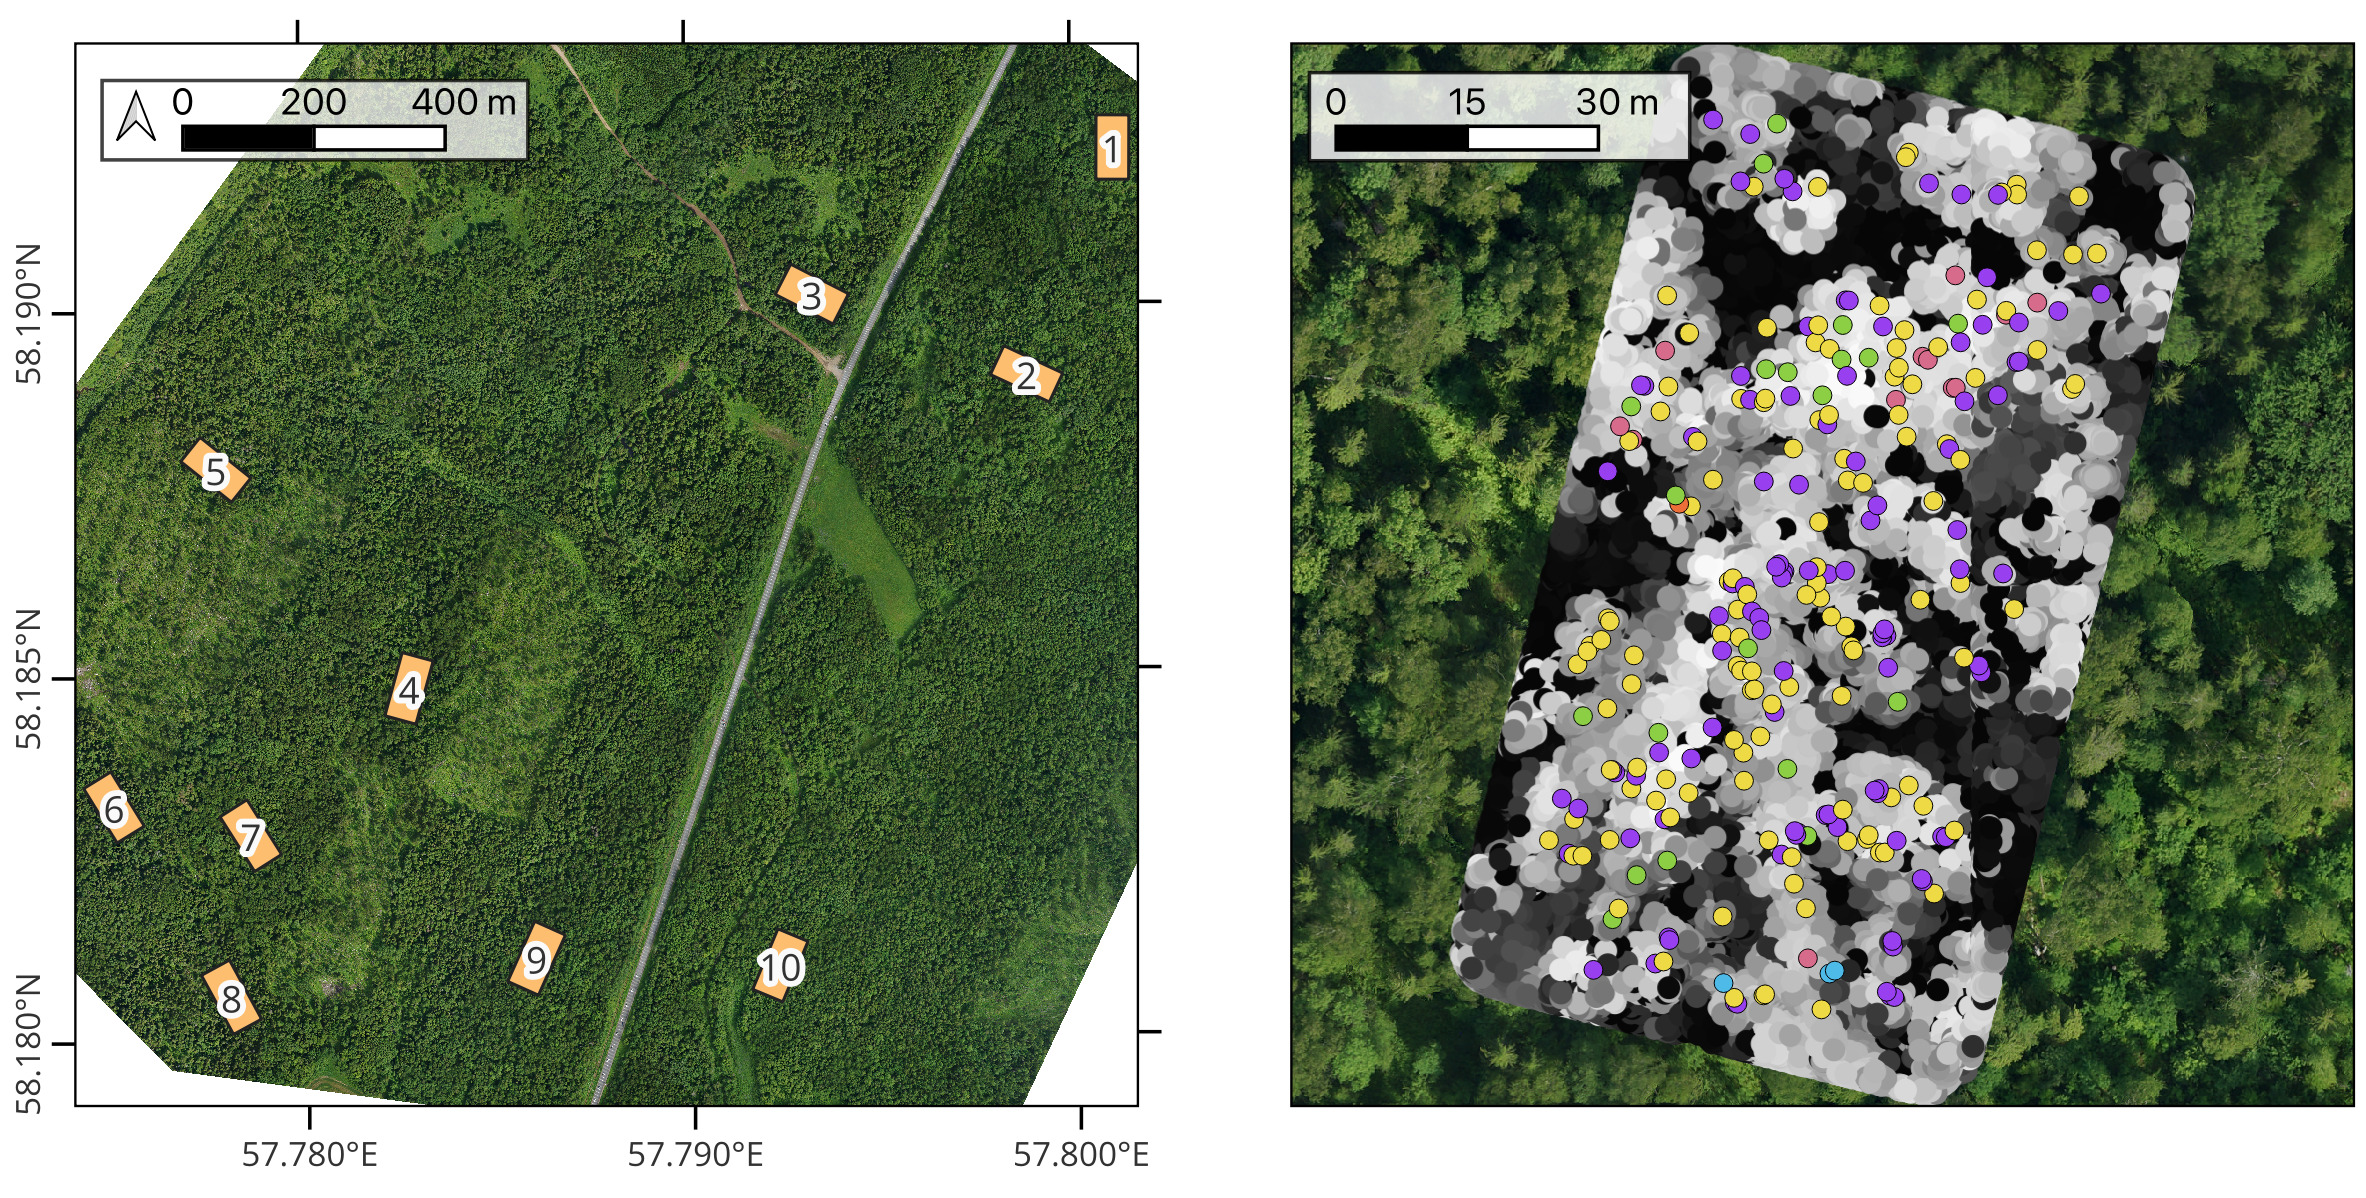
\includegraphics[width=\textwidth]{../images/lysva_roi.jpg}
}
\caption[The study region for the Lysva field inventory.]{\label{fig-lysva-roi}The study region for the Lysva field
inventory dataset. \textbf{Left}: The locations of field survey plot
boundaries on a full-size RGB orthophoto. Each plot is a 50 by 100 meter
rectangle, with every tree within measured and recorded. Buffered
cutouts of the orthophoto come with the dataset, along with LiDAR point
clouds. \textbf{Right}: A close up of plot number 4. Each colored point
represents a single tree of a different species, on top of a point cloud
colored by the value of the height of each point (lower points are dark,
higher points are bright) and the same orthophoto.
Note that the points of the point cloud are unsorted, and some lower points overlap higher points.
Figure reused from \citet{dubrovinOpenDatasetIndividual2024}.}
\end{figure}


The field inventory is a tabular dataset where every row represents a single tree.
Table~\ref{tbl-inventory-example} shows a random sample of entries from the field inventory table.
Every tree is represented by a point in UTM 40N coordinate reference system (EPSG:32640).
Every tree has a species label and diameter at breast height (dbh), measured with calipers at 1.3 m from the ground at two perpendicular directions and averaged.
Figure~\ref{fig-lysva-species-distribution} shows the distribution of species in the data: the dominant species is spruce, but overall the trees are evenly split between deciduous and coniferous, 1793 and 1807 respectively, with seven species in total: spruce, birch, fir, aspen, tilia, alder, and willow.
Approximately 20\% of the trees have height data measured during the inventory, and 10\% have ages measured on core samples, shown in the table in meters and years respectively.


\begin{longtable}[]{@{}lllllllllll@{}}

\caption[Example of data in the field inventory table.]{\label{tbl-inventory-example}Example of data in the field
inventory table. Each row is a recorded tree and is represented by a point un UTM 40N coordinate reference system (EPSG:32640). Coordinates are not shown.}

\tabularnewline

\toprule\noalign{}
Plot & Tree ID & Species & $d_1$ & $d_2$ & dbh & Age & Height & Angle &
Comment \\
\midrule\noalign{}
\endhead
\bottomrule\noalign{}
\endlastfoot
7.0 & 111.0 & Birch & 23.0 & 23.0 & 23.00 & – & – & 0.0 & – \\
5.0 & 136.0 & Fir & 23.5 & 23.0 & 23.25 & 90.0 & 17.5 & 0.0 & Rotten \\
3.0 & 119.0 & Aspen & 36.1 & 42.1 & 39.10 & 89.0 & 25.5 & 0.0 & – \\
9.0 & 345.0 & Spruce & 19.7 & 22.0 & 20.85 & – & 15.9 & 0.0 & – \\
6.0 & 267.0 & Spruce & 12.9 & 12.9 & 12.90 & – & – & 0.0 & – \\

\end{longtable}

\begin{figure}
\centering{
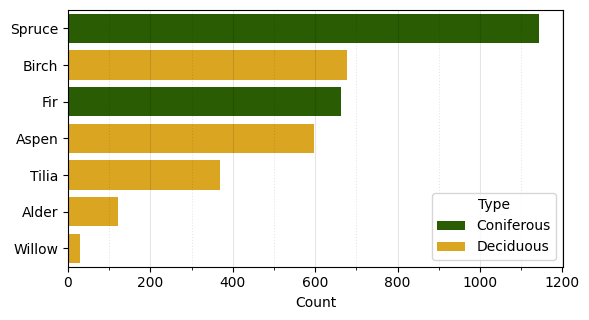
\includegraphics[width=\textwidth]{../images/03a_lysva_dataset-fig-lysva-species-distribution-output-1.png}
}
\caption[Distribution of species in the Lysva field inventory dataset]{\label{fig-lysva-species-distribution}Distribution of species
in the Lysva field inventory dataset. The dominant species is spruce,
but overall the split between coniferous and decidious species is even:
there are 1807 coniferous and 1793 deciduous trees.
Figure reused from \citet{dubrovinOpenDatasetIndividual2024}.}
\end{figure}

The LiDAR sensor used for the survey is AGM-MS3 produced by AGM Systems.
It has 640 kHz acquisition rate, 300-meter range, and spatial accuracy of 3–5 centimeters.
The raw point clouds were processed with the combination of the AGM ScanWorks software from the sensor vendor and the TerraScan software.
The point clouds were preprocessed by removing duplicate points and high and low noise points.
The duplicate removal was run with a threshold distance between points of 1 mm.
Noise was removed by visually inspecting the point cloud and manually selecting height thresholds to cut off points that are lower than the ground or higher than the canopies.
Ground point classification was performed and ground points were used to normalize height by subtracting the ground level from the Z coordinate of every point.
Height normalization allows treating the Z coordinate as height above ground rather than the absolute elevation, which simplifies many subsequent steps.
The camera used for the orthophoto survey is Sony A6000.
The resolution of the orthophoto is 7 centimeters per pixel.
Figure~\ref{fig-example-3d-point-cloud} is a 3D visualization of the point cloud over plot number 10.
It shows the unmodified point cloud on the left, with points colored by height above ground, and a point cloud enriched with color information by sampling the orthophoto at the planar coordinates of the points.
Figure~\ref{fig-example-ortho} shows the orthophoto for the same plot.
The carrier UAV was configured to follow the terrain at 150 meter height using the SRTM elevation map as a reference \citep{farrShuttleRadarTopography2000}.

\begin{figure}
\begin{minipage}{0.50\linewidth}
\centering{
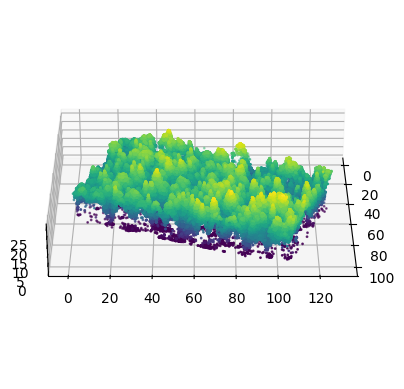
\includegraphics[width=\textwidth]{../images/03a_lysva_dataset-fig-example-3d-point-cloud-output-1.png}
}
\subcaption{\label{fig-example-3d-point-cloud-1}Points colored by
height.}
\end{minipage}
\begin{minipage}{0.50\linewidth}
\centering{
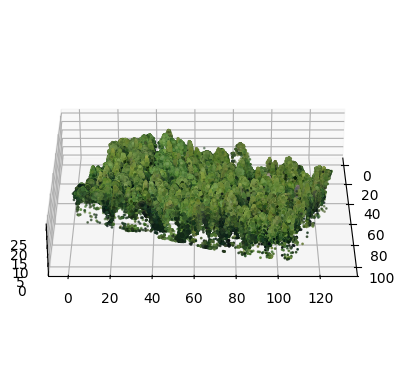
\includegraphics[width=\textwidth]{../images/03a_lysva_dataset-fig-example-3d-point-cloud-output-2.png}
}
\subcaption{\label{fig-example-3d-point-cloud-2}Points assigned color by
sampling the orthophoto.}
\end{minipage}
\caption{\label{fig-example-3d-point-cloud}A 3D visualization of the UAV
LiDAR point cloud of plot 10.}
\end{figure}

\begin{figure}
\centering{
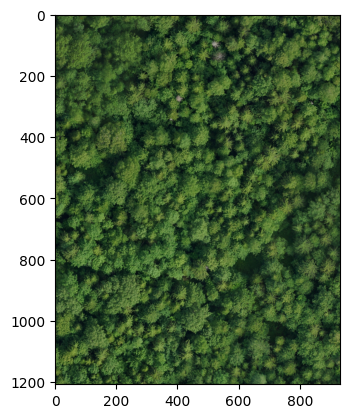
\includegraphics[width=\textwidth]{../images/03a_lysva_dataset-fig-example-ortho-output-1.png}
}
\caption{\label{fig-example-ortho}A visualization of the orthophoto of
plot 10.}
\end{figure}

Table~\ref{tbl-lysva-plot-stats} shows some descriptive statistics for each plot in the field inventory: the number of trees in the plot, average LiDAR point density in points per square meter, and dominant species type.
The overall average point density is 37 points per square meter.
Exactly half of the plots are predominantly coniferous and half are predominantly deciduous.
Figure~\ref{fig-lysva-canopy-structure} shows two point clouds clipped by plot bounds in 3D, highlighting the differences in canopy structure complexity between predominantly deciduous and coniferous plots.
The figure highlights that the forest is indeed dense and mixed, with non-uniform, complex canopy structure.

\begin{table}
    \centering
    \caption{\label{tbl-lysva-plot-stats}Statistics for the plots in the
Lysva dataset.}
    \begin{tabular}{llll}
    \toprule
Plot & Tree count & Point density & Dominant type \\
    \midrule
1.0 & 420 & 31.7 & Deciduous \\
2.0 & 365 & 47.9 & Deciduous \\
3.0 & 332 & 40.3 & Deciduous \\
4.0 & 261 & 33.5 & Coniferous \\
5.0 & 208 & 14.2 & Coniferous \\
6.0 & 290 & 39.1 & Coniferous \\
7.0 & 408 & 41.9 & Deciduous \\
8.0 & 341 & 35.5 & Coniferous \\
9.0 & 459 & 42.1 & Coniferous \\
10.0 & 518 & 42.9 & Deciduous \\
    \bottomrule
    \end{tabular}
\end{table}

\begin{figure}
\centering{
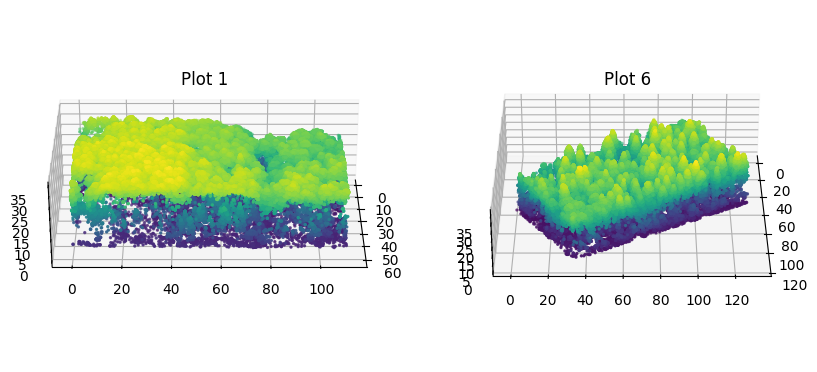
\includegraphics[width=\textwidth]{../images/03a_lysva_dataset-fig-lysva-canopy-structure-output-1.png}
}
\caption[Comparison of canopy structure in 3D point clouds.]{\label{fig-lysva-canopy-structure}3D visualizations of point
clouds from plot 1 (predominantly deciduous) and plot 6 (predominantly
coniferous). Note the difference in the canopy structure: it is
relatively easy to tell confifiers apart visually, while deciduous
species do not have pronounced shapes and are hard to discriminate.
Figure reused from (Dubrovin and Fortin 2024).}
\end{figure}

\subsubsection{On using intensity-based features}\label{sec-intensity-based-features}

Even though some sources report intensity-based features as some of the most important ones \cite{shiImportantLiDARMetrics2018}, the features seem to me unreliable in the context of forestry because of the physics of light reflection.
There are simply too many factors that affect the amplitude of the reflected signal, which might be useful when imaging stable targets such as urban environments but become completely unpredictable on highly unstable targets such as trees: they move in the wind in the time span of a single survey, they grow in the time span between repeated surveys, the leaves and branches are angled in every possible way.
Moreover, the quality of the recorded intensities highly depends on the used sensor.
As an example, Figure~\ref{fig-intensity-with-example} shows the distribution of intensity values for every point in the Lysva dataset, and shows plot number 10 in 3D with points colored by their recorded intensity.
The distribution of intensities seems like an artifact of faulty quantization (the fact that the maximum overall value is 63 makes me suspect it is stored by the hardware using a 6-bit unsigned integer, probably an ad hoc optimization by the sensor vendor).
With this distribution in mind, it is not surprising that coloring points by their intensity values results in images that look like noise, and there is no signal to be exploited for predictive modeling.

\begin{figure}
\begin{minipage}{0.50\linewidth}
\centering{
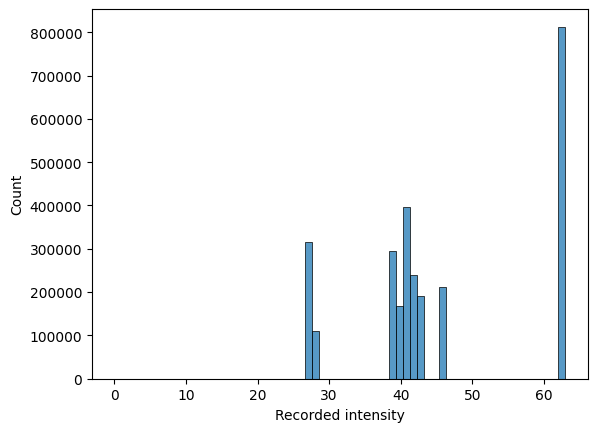
\includegraphics[width=\textwidth]{../images/03a_lysva_dataset-fig-intensity-with-example-output-1.png}
}
\subcaption{\label{fig-intensity-with-example-1}Distribution of
intensity over all points in the Lysva dataset.}
\end{minipage}
\begin{minipage}{0.50\linewidth}
\centering{
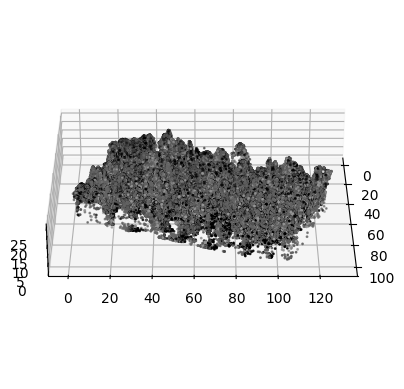
\includegraphics[width=\textwidth]{../images/03a_lysva_dataset-fig-intensity-with-example-output-2.png}
}
\subcaption{\label{fig-intensity-with-example-2}A point cloud of plot 10
with points colored by intensity.}
\end{minipage}
\caption{\label{fig-intensity-with-example}An example of the
unreliability of the intensity attribute.}
\end{figure}

Some sensors do provide more consistent values.
However, relying on intensity-based features limits the applicability of developed models and methods, as any such model would surely fail on data like this.

\subsubsection{Comparison to other datasets}

Our dataset is in many ways similar to the NewFor benchmark \cite{eysnAlpineITDBenchmark2015}.
It serves the same purpose and also offers overlapping field survey ground plots and UAV LiDAR point clouds.
There are, however, many notable differences.
The NewFor benchmark covers much more diverse regions, including ground plots from France, Italy, Switzerland, Austria, and Slovenia, while all our data comes from the same area.
The tree species covered by the datasets are also different: both contain spruce and fir, but the NewFor data also has beech, Scots pine, larch, sycamore, and poplar, while ours also has birch, aspen, tilia, alder, and willow.
Our dataset has more than twice as many individual trees as the Alpine benchmark, and the forest is denser and more complex, making it more complicated to detect trees in.
Our data contains very mild terrain variations, while the slopes of the terrain in Alpine data are very steep, which plays a role during height normalization, since subtraction of steep terrain introduces artificial slope to the points in the canopy, changing the overall shape of the tree.
Our dataset has an additional information source – an RGB orthophoto that allows development of algorithms that fuse multimodal data, which, we believe, is a key to success in such complex environments.
Our dataset has species labels for every surveyed tree, but only partial coverage of tree heights and no timber volume information at all.

Another similar dataset is the NeonTreeEvaluation Benchmark \cite{weinsteinDataNeonTreeEvaluationBenchmark2022}, which offers bounding box annotation for tree detection across a wide range of different forest types.
It offers coregistered RGB, LiDAR, and hyperspectral images over 31,000 individual trees.
The main difference in the reference data between the NeonTreeEvaluation Benchmark and our dataset is the source: our data comes from a field inventory and thus has additional tree information that can be used in downstream tasks, such as species classification or timber volume prediction, while the NeonTreeEvaluation Benchmark annotations are created from the RGB photo and thus only offer the positions and sized of trees.

Another dataset is the IDTReeS 2020 Competition Data \cite{gravesIDTReeS2020Competition2020} aimed to develop algorithms for delineation and species classification of individual tree crowns in RGB, LiDAR, and hyperspectral data.
It offers bounding box annotations for 1200 individual trees covered by RGB, LiDAR, and hyperspectral images in 3 national forests in the USA.
Similarly, the source of the data is annotation of images, not a field inventory.

There are also datasets available that do not have LiDAR point cloud coverage, or use terrestrial LiDAR instead of UAV LiDAR, or use photogrammetric point clouds instead of LiDAR  point clouds.
We do not mention them here because we specifically focus on UAV LiDAR.

\section{Individual tree point clouds dataset}\label{sec-individual-trees-dataset}

The main dataset used for training the models is a collection of point clouds of individual trees, sometimes referred to in this text as tree clouds, extracted manually from larger UAV LiDAR point clouds.
The dataset is released into open access, and was originally presented in \citep{dubrovinExplorationPropertiesPoint2024}, although it has been expanded since and now contains twice as many individual trees.
It consists of 394 trees, 192 of which are extracted from the previously described Lysva survey, and 202 from other surveys in Perm Krai.
The distinction between the parts is important because the Lysva dataset has RGB orthophoto coverage, making it possible to infuse the tree clouds with orthophoto-based features.
Thus, for training the tree segmentation networks that rely on these features, the effective size of the dataset is 192 tree clouds, as only the former part is used.
However, the whole dataset is used for training regression and classification models that process segmented trees.

Figure~\ref{fig-individual-trees-species-distribution} shows the distribution of species in the individual tree point clouds dataset.
The split between coniferous and deciduous trees is almost even: there are 202 coniferous and 193 deciduous trees.
There are seven species in total: spruce, birch, aspen, pine, fir, alder, and tilia, with most focus on 4 most important species listed first.
Note the presence of pine trees, which are not present in the Lysva field inventory data, and the absence of willow trees.
All the pine trees are from other field surveys.
Willows are skipped intentionally, since they are of little interest in terms of timber harvesting: they are considered low quality, and their ripening cycle is mismatched with main timber species – when the overall plot is ready to be harvested, the willows are already rotten.

\begin{figure}
\centering{
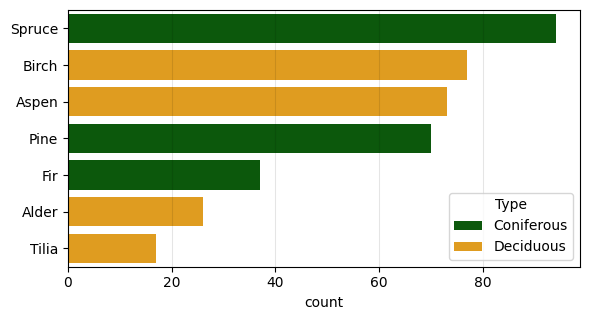
\includegraphics[width=\textwidth]{../images/03b_individual_trees-fig-individual-trees-species-distribution-output-1.png}
}
\caption[Distribution of tree species in the individual trees dataset]{\label{fig-individual-trees-species-distribution}Distribution
of tree species in the individual trees dataset. It contains 394 point
clouds of individual trees: 201 coniferous and 193 deciduous. Note the
presence of pine trees, as there are no pine trees in the Lysva field
inventory -- all of the pines come from other field surveys.}
\end{figure}


Figure~\ref{fig-individual-trees-visualization} is a visualization of the data.
It shows a random tree of every species as a 2D scatter plot and a single spruce as a 3D scatter plot with points colored by height.
Because the observations are made from above, many trees have the highest concentrations of points at the top of their canopy and a very limited number of points along the trunk.
Additionally, slight slopes of the terrain manifest as artificial tilt in some of the trees because of the height normalization of the original point cloud.

\begin{figure}
\begin{minipage}{0.7\linewidth}
\centering{
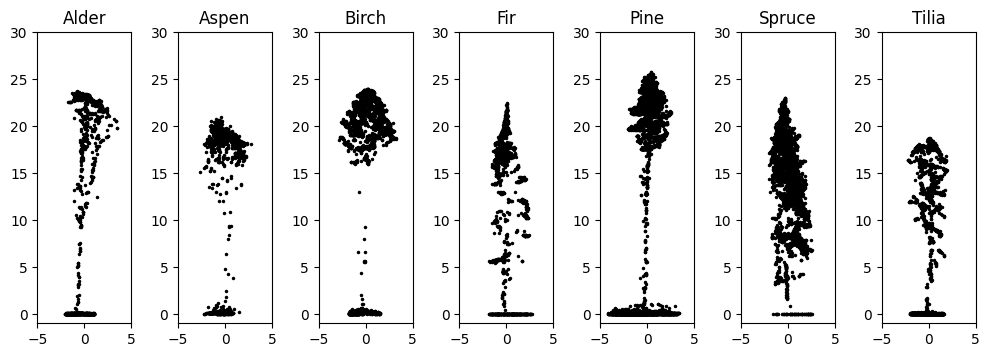
\includegraphics[width=\textwidth]{../images/03b_individual_trees-fig-individual-trees-visualization-output-1.png}
}
\subcaption{\label{fig-individual-trees-visualization-1}Cross-sections
of random trees of every species (ignoring the Y dimension).}
\end{minipage}
\begin{minipage}{0.29\linewidth}
\centering{
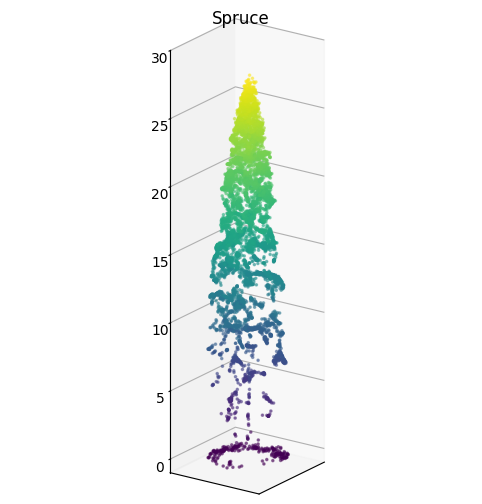
\includegraphics[width=\textwidth]{../images/03b_individual_trees-fig-individual-trees-visualization-output-2.png}
}
\subcaption{\label{fig-individual-trees-visualization-2}A spruce in 3D.}
\end{minipage}
\caption[Visualizations of the individual tree point clouds in the dataset.]{\label{fig-individual-trees-visualization}Visualizations of the
individual tree point clouds in the dataset. Most of the tree clouds are
top-heavy because of the observation from above, and some are
artificially tilted because of slight terrain slopes and height
normalization. The ground points are present.}
\end{figure}

An important note is that the extracted trees were not chosen for extraction randomly but were selected by humans based on whether it was possible and relatively easy to separate from the surrounding trees.
So there is a selection bias in there favoring the trees that are easily separable, standing outside of large dense clusters.
Because of that the trees do not exactly represent what a tree closely surrounded by other trees is like in a point cloud.
It is especially apparent in very pronounced trunks of all the visualized trees.
In a dense forest, such as the one visualized in Figure~\ref{fig-lysva-canopy-structure}, there is hardly ever enough penetration for such detailed trunk coverage.
In fact, as mentioned in the literature review, good coverage of trunks is an immensely useful feature of terrestrial LiDAR surveys, which consistently show very good results using algorithm that segment trees from the trunk up.

\section{Synthetic forests generated from individual trees}\label{sec-synthetic-forest-dataset}

To train tree segmentation models, training data where every point is assigned to an individual tree is required.
Data like that are very labor-intensive to label.
An alternative way to create such data is by generating it from a set of tree clouds, as the per point labels arise naturally in this case.
I used the dataset of individual tree point clouds described in the previous section to generate a synthetic forest to train a tree segmentation PointNet++.

Synthetic forest is generated in patches of set height and width by sampling individual trees from the full set and placing them from left to right, until the set width is extended, then from bottom to top, until the set height is extended.
A height threshold is applied to each tree before placing it to remove ground points and non-tree reflections.
This results in patches that are slightly bigger than the set size, but that can be cropped into the exact size.
This has an added benefit of mimicking cutoff trees at the edges of the patch that are inevitable when the model is applied in a sliding window.
The trees can be sampled with or without replacement, but since a set of augmentations described in Section~\ref{sec-augmentations} is applied to each tree individually, exact same tree never occurs in the patch fed to the model even when sampling with replacement.
When trees are placed, their planar bounding boxes are tracked to avoid overlap.
However, since some overlap might, in fact, be desired to better represent actual forests, a parameter that controls the amount of overlap is added to the dataset generation process.
Each tree is also assigned a label, which simply tracks its ordinal number in the patch.
An example of a 20 by 20 meter synthetic forest patch with 0.75 meter overlap and 2 meter height threshold is shown in Figure~\ref{fig-synthetic-forest-patch-example} from two different perspectives and using two color schemes: the label, i.e. the ordinal ID of the tree within a patch, and RGB color sampled from the orthophoto.

\begin{figure}
\centering{
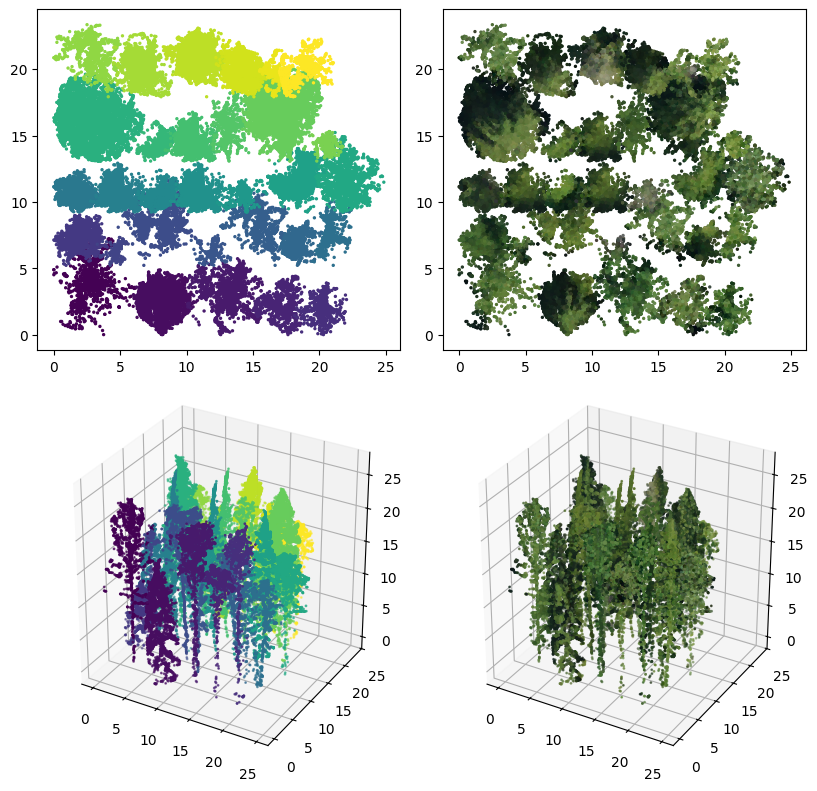
\includegraphics[width=\textwidth]{../images/03c_synthetic_forest-fig-synthetic-forest-patch-example-output-1.png}
}
\caption[Visualisation of a synthetic forest patch used for
training]{\label{fig-synthetic-forest-patch-example}A visualization of a
synthetic forest patch used for training the tree segmentation network.
Patch width and height are set to 20 meters, overlap is set to 0.75.
\textbf{Top:} Top-down view of the patch. \textbf{Bottom:} 3D view of
the same patch. \textbf{Left:} Points colored by label: unique tree ID
within the patch. \textbf{Right:} Points colored by RGB color sampled
from the orthophoto.}
\end{figure}

For comparison, a patch of the same size from a real point cloud over one of the plots of the Lysva survey is shown in Figure~\ref{fig-lysva-plot-window-example}.

\begin{figure}
\centering{
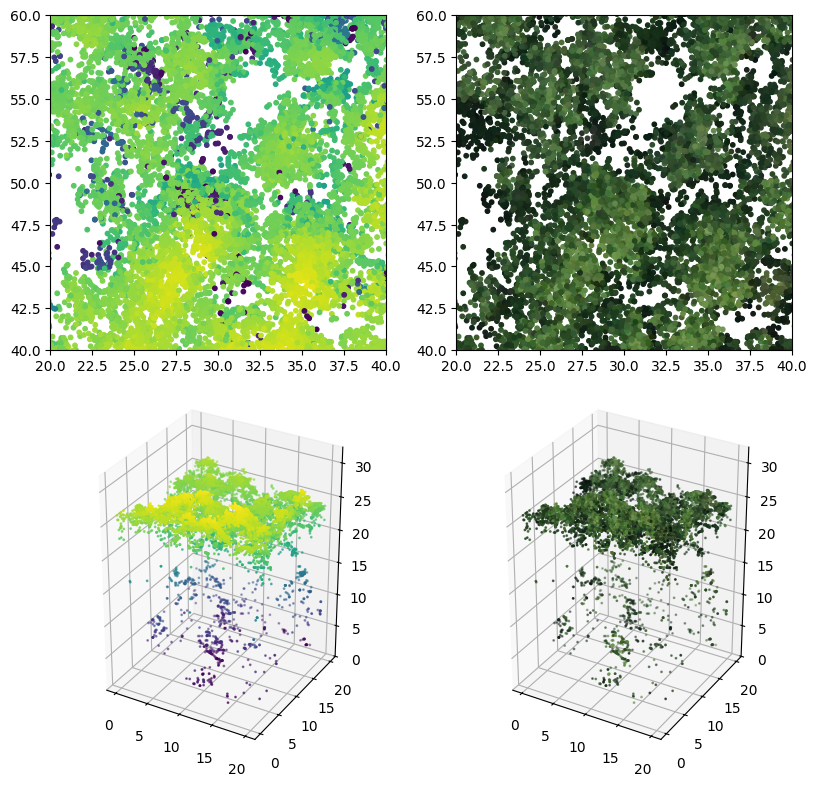
\includegraphics[width=\textwidth]{../images/03c_synthetic_forest-fig-lysva-plot-window-example-output-1.png}
}
\caption[Visualisation of a patch of a real forest.]{\label{fig-lysva-plot-window-example}A piece of the Lysva
LiDAR point cloud over plot 10 in within a 20 by 20 meter window.
\textbf{Top:} Top-down view. \textbf{Bottom:} The same patch in 3D view.
\textbf{Left:} Points colored by height. \textbf{Right:} Points colored
by RGB color sampled from the orthophoto.}
\end{figure}

An alternative approach to creating patches of synthetic forest can be to use a fixed number of trees instead of fixed patch size.
However, it poorly correlates with how the final model will be applied: in windows of fixed size, not windows with varying size but fixed number of trees.
And size of the patch the model sees is important because the scale is normalized, and using a different patch sizes changes the scaled coordinates and confuses the model that learned to rely on them.

Enriching point clouds using only color information from RGB orthophotos provides limited utility because it adds only local information to the points.
As was mentioned in the introduction, one of the aspects of the complementary nature of the two data sources is that images provide continuous representations and capture textures.
To enrich the image features with context, they can be preprocessed with feature extractors that encode context into pixel values and thus provide more information for the segmentation network.
The feature extractors can be simple algorithms or specialized convolutional network feature extractors.
For the same reason a simple PointNet++ is used as the architecture for the tree segmentation network, a simple collection of multi-scale features are used as orthophoto features, including intensity, edge, and texture features, extracted from the orthophotos using the \texttt{scikit-image} Python package.
The features are calculated on different scales by applying Gaussian smoothing with varying parameters before calculation.
Figure~\ref{fig-basic-features-small} shows example features from every mentioned group on a very fine scale.
The top left image is the original orthophoto of plot 10 from the Lysva survey, the top right image is the intensity calculated from it, and bottom images are examples of an edge feature and a texture feature.
The same features but on a coarser scale are shown in Figure~\ref{fig-basic-features-large}.

\begin{figure}
\centering{
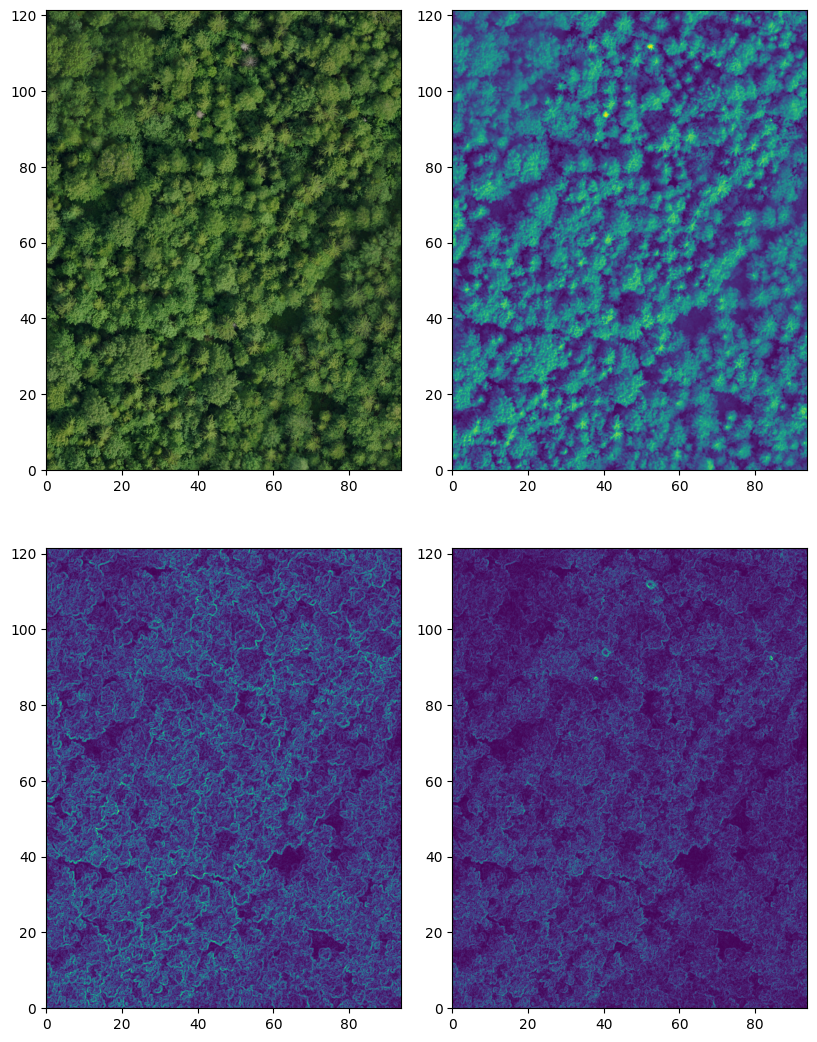
\includegraphics[width=\textwidth]{../images/03c_synthetic_forest-fig-basic-features-small-output-1.png}
}
\caption[Visualisation of basic orthophoto-based features (small
scale)]{\label{fig-basic-features-small}Basic orthophoto-based features
used (on a single scale with sigma=1, actual features are across
multiple increasing scales). \textbf{Top left}: The original orthophoto
for plot 10. \textbf{Top right}: Intensity feature. \textbf{Bottom
left}: Edges feature. \textbf{Bottom right}: Texture feature.}
\end{figure}

\begin{figure}
\centering{
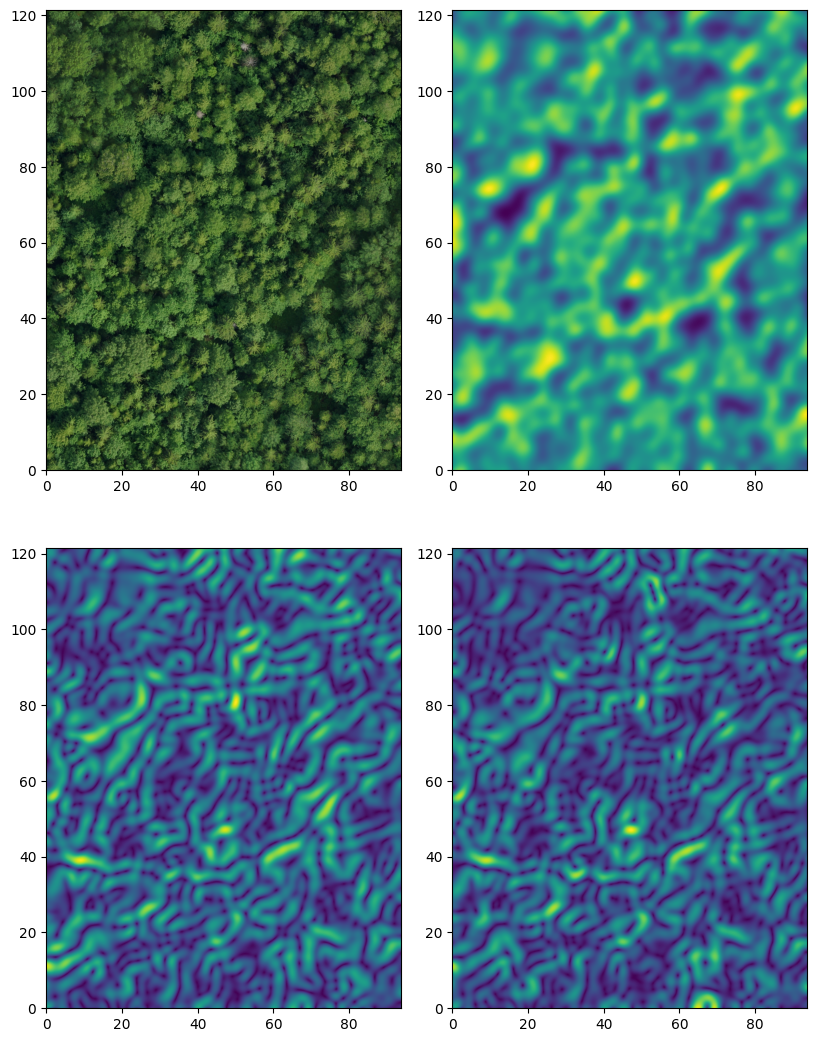
\includegraphics[width=\textwidth]{../images/03c_synthetic_forest-fig-basic-features-large-output-1.png}
}
\caption[Visualisation of basic orthophoto-based features (large
scale)]{\label{fig-basic-features-large}Basic orthophoto-based features
used (on a single scale with sigma=16, actual features are across
multiple increasing scales). \textbf{Top left}: The original orthophoto
for plot 10. \textbf{Top right}: Intensity feature. \textbf{Bottom
left}: Edges feature. \textbf{Bottom right}: Texture feature.}
\end{figure}

\section{Training tree segmentation neural networks}

The architecture chosen to serve as the tree segmentation network is the PointNet++ \citep{qiPointNetPlusPlus2017}, described in detail in Section~\ref{sec-ml-dl}.
It is a relatively simple architecture, and further potential quality improvements might be achieved by using more modern and advanced architectures instead.
However, the main goal of this thesis was to develop and verify an overall framework, and thus the choice was set on a model that is simple to implement and work with to allow easy experimentation with other parts of the proposed system.

The architecture of the used PointNet++ is similar to the segmentation architecture shown in Figure~\ref{fig-pointnet2-architecture}.
The main differences from the shown architecture are the use of one more stacked set abstraction layer to make the network deeper, and the use of a regression head that predicts a continuous value for each point instead of a classification head that predicts per-point class scores, since the model needs to assign a unique ID to every tree in the patch.
The three stacked set abstraction layers have the proportions of points sampled set to 0.75, 0.5, and 0.5, and neighborhood radii for feature aggregation set to 0.1, 0.2, and 0.4.
Note that the scale of the input is normalized (see next subsection for details), so the radii are not in meters.
The model has 30 million trainable parameters.

\subsection{Coordinate and feature normalization}

It's a well established practice to scale the inputs to neural networks that is known to improve the speed and accuracy of gradient descent convergence \citep{bishop2006pattern}.
Before going through the network, a set of augmentations and transformations is applied to each synthetic forest patch.
The augmentations are described in detail with visualized examples in Section~\ref{sec-augmentations}.
The transformations include scale and feature normalization – the coordinates are centered and normalized to the interval $(-1, 1)$ and the features are normalized to the interval $(-1, 1)$ without centering.

\subsection{Data augmentation}\label{sec-augmentations}

The primary objective of data augmentation is to enhance the quantity, quality, and variety of data used for training \citep{mumuniDataAugmentationComprehensive2022}.
This is especially important when the sizes of the available datasets are limited, like in the case of the individual trees data that is the base of the synthetic forest datasets.
Carefully selected augmentations allow increasing the effective dataset size.
However, it is important to pay attention that the chosen augmentations keep the transformed examples semantically equivalent to the original.
A readily understandable example of a bad augmentation in the task of digit classification, which is often used as the "hello world" of deep learning with the MNIST dataset of handwritten digits \citep{deng2012mnist}, is a vertical flip, as most digits lose meaning when upside down.
A flip is also a bad augmentation example for a synthetic forest patch described in Section~\ref{sec-synthetic-forest-dataset}, as it changes the order of the trees within a patch, thus breaking the labels that are assumed to increase in a specific pattern.

In the scenario when the data for is created by combining several smaller inputs, there is a possibility of applying augmentations on two different scales.
The most simple approach is to treat a synthetic forest patch as a whole and apply augmentations directly to it.
However, it is also possible to apply per-tree augmentations, effectively increasing the size of the underlying tree set from which synthetic forest patches constructed.
Only the latter kind are used for training the tree segmentation network.

The first transformation that changes the shape but does not affect any semantics for an individual tree is a random rotation around the vertical axis.
A tree remains completely the same when rotated, but the coordinates of all points change.
Figure~\ref{fig-random-rotate-effect} shows the effect of applying random rotation transformation of different magnitudes to a single aspen tree.
For visualization purposes, the rotation is forced to apply with full magnitude for every parameter.
During training, the angle is uniformly sampled from the specified range.
For the final tree segmentation model, the range is set to $[-180, 180]$ degrees, as no amount of rotation breaks the semantics.

\begin{figure}
\centering{
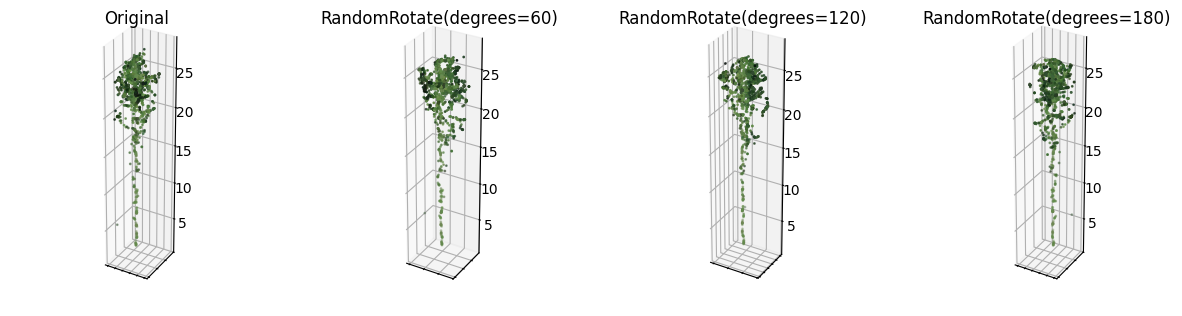
\includegraphics[width=\textwidth]{../images/03d_augmentations-fig-random-rotate-effect-output-1.png}
}
\caption[Visualization of the random rotation around Z axis augmentation on a single aspen tree.]{\label{fig-random-rotate-effect}Visualization of the random
rotation around Z axis augmentation on a single aspen tree. The effect
is forced to happen with full amplitude for visualization purposes,
during training a rotation angle is uniformly sampled from a set range.}
\end{figure}%

Another transformation that keeps the tree the same but changes the coordinates of the points is random scaling.
It simply multiplies the coordinates by a scaling factor, making the tree larger or smaller in all directions.
Unlike random rotation around the vertical axis, however, the range needs to be chosen much more carefully, as there is a possibility of making unrealistically large or small trees that would confuse the model during training.
Figure~\ref{fig-random-scale-effect} shows the effect of applying random scale transformation to a single aspen tree.
Again, for purposes of visualization, the scale is forced to apply with full magnitude.
During training, the scale is uniformly sampled from the specified range.
For the final tree segmentation model, the range is set to $[0.8, 1.2]$.

\begin{figure}
\centering{
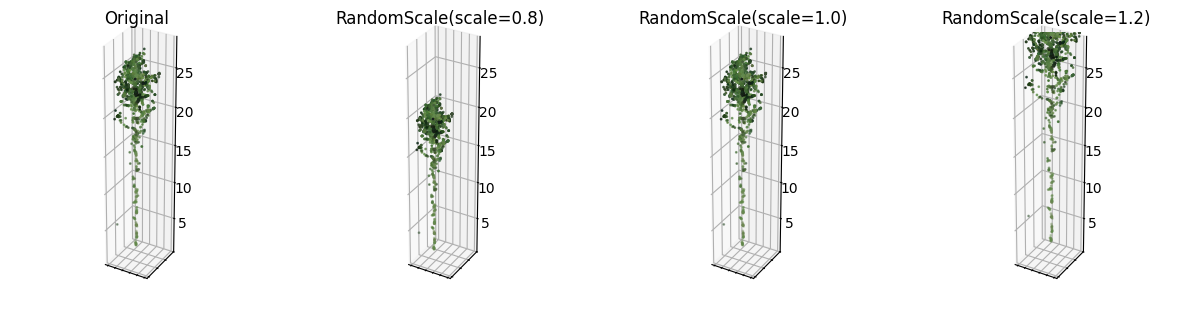
\includegraphics[width=\textwidth]{../images/03d_augmentations-fig-random-scale-effect-output-1.png}
}
\caption[Visualization of the random scale augmentation on a single aspen tree.]{\label{fig-random-scale-effect}Visualization of the random
scale augmentation on a single aspen tree. The effect is forced to
happen with full amplitude for visualization purposes, during training a
scale factor is uniformly sampled from a set range.}
\end{figure}

Another way to change the positions is to slightly translate each point for a random distance in a random direction.
That transformation is commonly referred to as random jitter.
Since LiDAR sensors have limited spatial accuracy, introducing random translations within the accuracy range should not have any effect on the result of tree segmentation.
Going further, small translations even outside the accuracy range make sense, since they have very limited effect on the overall shape of the tree.
Figure~\ref{fig-random-jitter-effect} shows this effect on a single aspen tree.
The amount of translation is uniformly sampled independently for each point from a set range.
Note that the random jitter augmentation is applied before the scale normalization.
It matters because the augmentation's only parameter is the translation range, which depends on the scale.
The parameters on the figure are thus in the original coordinate units – meters.
Note how the shape of the tree almost does not change when the maximum range is set to 20 centimeters, and starts to become fuzzy and loose shape at 1 meter and higher.
For the final tree segmentation model, the maximum translation is set to 30 centimeters.

\begin{figure}
\centering{
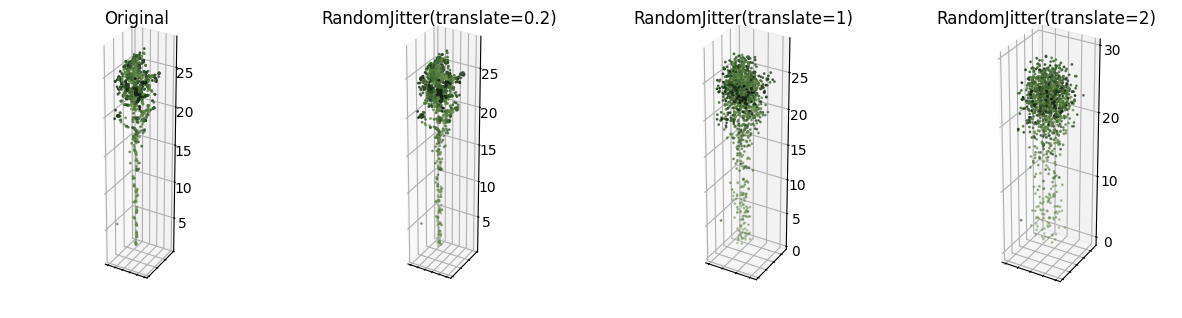
\includegraphics[width=\textwidth]{../images/03d_augmentations-fig-random-jitter-effect-output-1.png}
}
\caption[Visualization of the random jitter augmentation on a single aspen tree.]{\label{fig-random-jitter-effect}Visualization of the random
jitter augmentation on a single aspen tree. The translation magnitude is
uniformly sampled from a set range for every point.}
\end{figure}

Another useful effect augmentations can provide is to make synthetic data look more like real data.
As was mentioned in Section~\ref{sec-individual-trees-dataset}, there is a selection bias in the dataset of individual trees: the trees that are easiest to manually separate are exponentially more likely to end up in the data.
As such, the tree clouds in the individual tree dataset are significantly different from trees of the same species with similar sizes and shapes, but standing in dense clusters.
One of the most important differences is that almost all the tree clouds have trunks, while in actual forest, dense canopy cover blocks most pulses and the trunk representation is very poor.
One way to mitigate that issue is to apply a height-dependent dropout function to each tree cloud.
For that purpose a probability threshold function that is around zero for the highest points of the tree and quickly ramps up to almost one for the lowest points is needed.
An example function that satisfies these criteria is a modified sigmoid:

$$
\text{threshold}(z) = \big[1 + e^{z \times \text{scale} + \text{shift}}\big]^{-1},
$$

where $z$ is the height normalized to $[0, 1]$ and reversed by subtraction from 1, $\text{scale}$ and $\text{shift}$ are hyperparameters that control the shape of the curve.
Changing $\text{scale}$ controls how steep is the climb from 0 to 1: the larger, the steeper.
Changing $\text{shift}$ controls the position of the climb: the larger, the lower.
Figure~\ref{fig-height-dropout} shows an example of applying such dropout function to a single aspen tree, and Figure~\ref{fig-height-dropout-aggressive} show the same tree with more aggressive parameters, resulting in much more points being dropped from the tree cloud.

\begin{figure}
\centering{
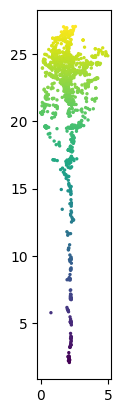
\includegraphics[width=\textwidth]{../images/03d_augmentations-fig-height-dropout-output-1.png}
}
\caption[Effect of the height-dependent modified sigmoid dropout on a single aspen tree.]{\label{fig-height-dropout}Effect of the height-dependent
modified sigmoid dropout on a single aspen tree. Scale is set to 8,
shift is set to 3. \textbf{a)} A single aspen tree with points colored
by height. \textbf{b)} Height-dependent probability of dropout (a
modified sigmoid). \textbf{c)} The same aspen with points colored by
probability of dropout. \textbf{d)} The same aspen with points that will
be dropped marked red. \textbf{e)} The same aspen after the dropout is
appleid with point colored by height.}
\end{figure}

\begin{figure}
\centering{
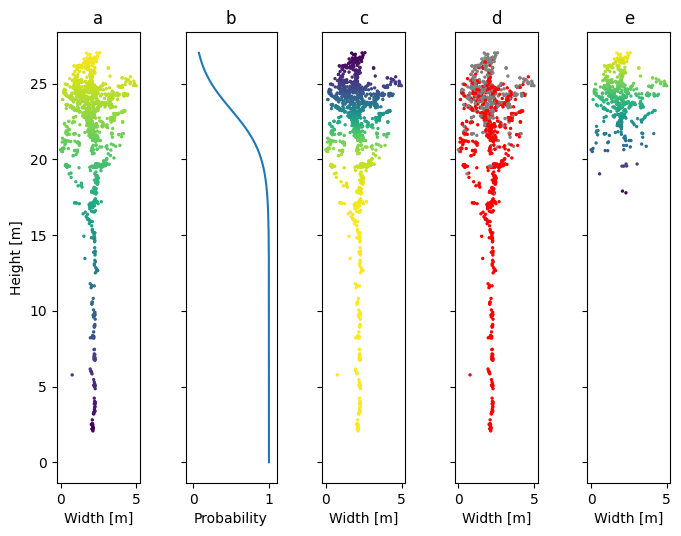
\includegraphics[width=\textwidth]{../images/03d_augmentations-fig-height-dropout-aggressive-output-1.png}
}
\caption[Effect of a stronger height-dependent modified sigmoid dropout on a single aspen tree.]{\label{fig-height-dropout-aggressive}Same as
Figure~\ref{fig-height-dropout}, but with a more aggressive dropout
threshold function. Scale is set to 18, shift is set to 2.5.}
\end{figure}

All the augmentation are applied on the fly right before the examples are loaded into GPU memory and passed through the network.

\subsection{Other training parameters}\label{sec-other-training-params}

Mean absolute error is used as a loss function.
Some experiments have shown improvements when using a custom loss function that modifies the mean absolute error loss by weighting it reversely proportional to the distance of the tree centroid.
The idea of the modification is to make the network focus more on points closer to the center of each tree, as these points are much less likely to be overlapping with the crowns of adjacent trees.

The batch size is limited by the available GPU device memory, and in the described setup competes for memory space with the synthetic forest patch dimensions used in the training dataset.
The preference is given to the size of the patch, so the batch size is set to 1, but is compensated for by using gradient accumulation steps – updates to the model parameters are made after the gradient is accumulated for a set number of iterations.
This slows down the training, but enables usage of larger batches when there is not enough memory to fit them, making the training procedure overall more stable.

Early stopping \citep{precheltAutomaticEarlyStopping1998} is set up to terminate training early if there is no improvement in average validation loss in a set number of epochs.
This makes sure that valuable GPU time is not wasted on continuing training models that are likely to have started overfitting.

Model checkpointing is set up as well.
After each training epoch, when the average validation loss and accuracy are calculated, the model state is saved to disk if it's current accuracy is better than the last saved one, where accuracy is the proportion of points for which the rounded integer label is correct.
This makes sure that the best performing model can always be recovered, even if the training process was run for too long and the latest model is not the best one.

The learning rate schedule is set to follow a fast linear warm up and slow linear decay.
Learning rate is set to ramp up from 0.001 to 0.01 in a span of 2 epochs, and then decay back to 0.001 in a span of 30 epochs.
Adam optimizer is used \citep{kingmaAdamMethodStochastic2014}.

Training was performed on an NVIDIA A100 GPU with 80 Gb of memory.
Inference, depending on the point density of the input, might work even on a much smaller GPU like Tesla T4 with 16 Gb of memory.
GPUs of this size are available with limits on usage for free on services like Google Colab and Kaggle.

\subsection{On implementation of PointNet++}

As mentioned in the introduction, the deep learning code, including the code for PointNet++, is implemented using the PyTorch Geometric library designed for writing and training graph neural networks.
This makes the implementation not exactly the same as described in the PointNet papers.
The main ideas, namely local feature learning in a k-nearest neighbors neighborhood and max pooling for permutation-invariant aggregation, are there.
Input transform and feature transform networks are not defined explicitly, but networks that process features learn to perform a similar function.

\section{Training segmented trees processing models}\label{sec-training-tree-processors}

To predict per-tree forest attributes from a segmented point cloud, a set of specialized regression and classification models is trained on the tree clouds.
These specialized models are classic machine learning models that operate on most common metrics described in the literature overview chapter.
As mentioned in the literature overview, common features used for machine learning on point clouds are based on the eigenvalues of the covariance matrix of the point coordinates, calculated either for an entire cloud, or per-point in a neighborhood around it.
These features include linearity, planarity, scatter, that aim to indicate the presence of linear, planar, or volumetric structures, and also omnivariance, anisotropy, eigentropy, the sum of eigenvalues, and curvature.
The features are defined as follows, with eigenvalues sorted in descending order such that $\lambda_1 \ge \lambda_2 \ge \lambda_3$:

$$
\begin{aligned}
\text{linearity} &= \frac{\lambda_1 - \lambda_2}{\lambda_1} \\
\text{planarity} &= \frac{\lambda_2 - \lambda_3}{\lambda_1} \\
\text{scatter} &= \frac{\lambda_3}{\lambda_1}  \\
\text{omnivariance} &= \sqrt[3]{\lambda_1\lambda_2\lambda_3} \\
\text{anisotropy} &= \frac{\lambda_1 - \lambda_3}{\lambda_1} \\
\text{eigentropy} &= -\sum_{i=1}^{3} \lambda_i \ln(\lambda_i) \\
\text{sum of eigenvalues} &= \lambda_1 + \lambda_2 + \lambda_3 \\
\text{curvature} &= \frac{\lambda_3}{\lambda_1 + \lambda_2 + \lambda_3} \\
\end{aligned}
$$

Another common set of features, especially popular in forestry applications, are various statistics that describe the height distribution of points within the neighborhood or the cloud.
They include maximum and average height, standard deviation, kurtosis, skew, and entropy of the height distribution, percentage of points above the mean and each of the deciles of height and the deciles of height themselves.
The features are calculated for the entire tree cloud, effectively reducing each tree to a collection of metrics, resulting in a tabular dataset.
In this form, the dataset is used to train the models.

In \citet{dubrovinExplorationPropertiesPoint2024}, we propose a way to help build intuition into the meaning of some of the less obvious features by visualizing individual trees on a different end of the range of the feature's values.
Figure~\ref{fig-feature-ranges} shows is an example of such visualization, showing the effect of the shape of spruce on omnivariance and the effect of the shape of aspen on percent of points above mean height.
Note the presence of ground points, which are filtered out before calculating features for the models.

\begin{figure}
\centering{
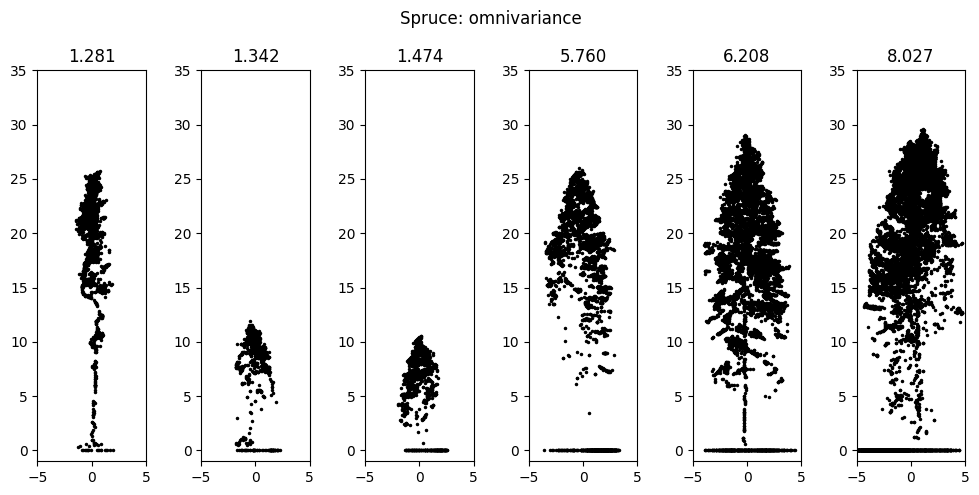
\includegraphics[width=\textwidth]{../images/fig-feature-ranges-output-1.png}
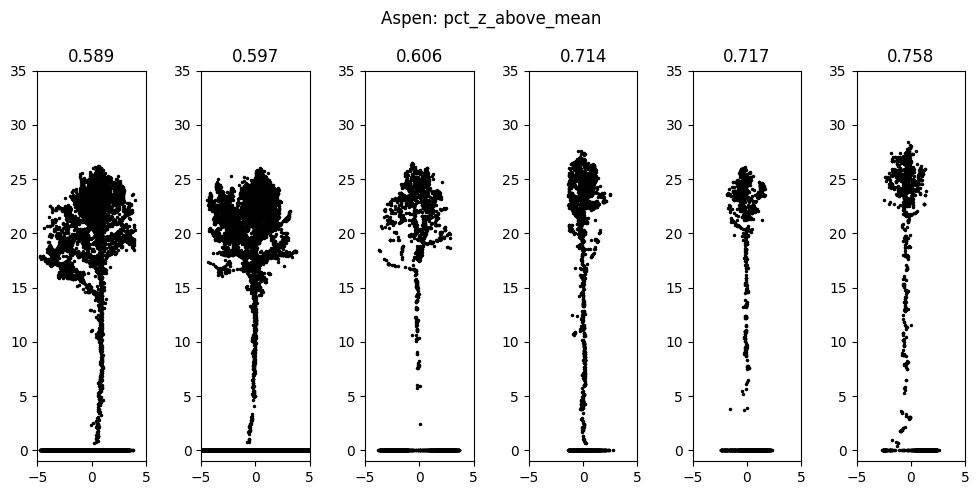
\includegraphics[width=\textwidth]{../images/fig-feature-ranges-output-2.png}
}
\caption[Visualizations of tree shapes at different ends of feature value ranges.]{\label{fig-feature-ranges}Visualizations of how values of
commonly used features calculated for the whole tree cloud map to the
shapes of individual trees. \textbf{Top}: Effect of the shape of spruce
on omnivariance. \textbf{Bottom}: Effect of on the shape of aspen on
percent of points higher than mean height. Figure reused from Dubrovin
and Fortin (2024). Note the presence of ground points, which are
filtered out before calculating features for the models.}
\end{figure}

The feature set is thinned by using sequential feature selection: a greedy approach that selects the best feature according to 5-fold cross-validation accuracy on every iteration until a set number of features is selected.
The models are trained on 20 best features selected this way.

To make the trees more closely resemble the trees standing in dense clusters, the same height-dependent dropout function that is used for augmenting synthetic forests is used.
This dropout, together with a small amount of random jitter, is also used to create additional samples for training the models, as the original dataset size is very small.
Great care is taken to only create additional samples within the training set, to avoid any data leakage.
Every training set sample is repeated 3 times with random jitter with maximum amplitude of 20 cm and a dropout applied.

Two models are used as proof of concept for the proposed framework: a classifier that predicts the tree species, and a regressor that estimates a tree's diameter at breast height.
Random Forest models are used in both cases.
The number of trees is set to 200.
For the classification model, class weights are assigned to every example that are inversely proportional to the class frequency in the data during model fitting.

\section{Matching detected trees to ground truth}\label{sec-matching-algorithm}

To evaluate the results of any tree detection system against field inventory data, an automated and deterministic method for matching detected tree candidates to the ground truth trees is needed.
It should determine which ground truth trees, if any, the detected candidates correspond to.
It should also classify both the trees and the candidates as either a true positive, meaning that the ground truth tree was successfully detected, a false negative, meaning that a ground truth tree was not detected, or a false positive, meaning a tree was detected when there is none.

I use the same matching procedure that is described and implemented in \citet{dubrovinOpenDatasetIndividual2024}.
It considers the locations and heights of the trees, and falls back to using only locations when the height is not available for the ground truth tree.
It is parametrized by the maximum allowed 2D distance and the maximum height difference between a detected and a ground truth tree to consider them a match.
First, it constructs a distance matrix between the ground truth tree locations and the detected candidates and filters out the pairs for which the distance is larger than the allowed maximum.
It then iterates over the remaining pairs in the order of increasing distance, and marks the pairs with suitable heights in which both trees are not yet assigned a class as a true positive.
The pairs in which one of the trees is already assigned a class are marked as either a false positive or a false negative, and the pairs in which both trees are assigned a class are skipped.
Finally, it marks all unmatched ground truth trees as false negatives, and all unmatched candidate trees as false positives.

Based on the results of the matching algorithm, a set of metrics that are often used to evaluate the results of tree detection can be calculated.
The same metrics are usually used for evaluation in classification problems and thus are well-known.
The first commonly used metric is recall, which is the proportion of the ground truth trees that were detected.
The second metric is precision, which is the proportion of candidates that are correct.
Both are important, and describe a detection system from different perspectives.
To combine them into a single metric, $F_1$-score is often used, which is the harmonic mean of precision and recall that provide a balanced measure of the system performance.
The formulas for the metrics are as follows:

$$
\text{recall} =
\frac{N_{\text{true positives}}}{N_\text{trees}} =
\frac{N_{\text{true positives}}}{N_{\text{true positives}} + N_{\text{false negatives}}}
$$

$$
\text{precision} =
\frac{N_{\text{true positives}}}{N_\text{candidates}} =
\frac{N_{\text{true positives}}}{N_{\text{true positives}} + N_{\text{false positive}}}
$$

$$
F_1\text{-score} = 2 \times \frac{\text{precision} \times \text{recall}}{\text{precision} + \text{recall}}
$$

Another commonly used metric to evaluate the results of tree detection approaches is the average distance between a detected and a ground truth tree.
This metric, however, has limitations that are important to keep in mind when analyzing the results.
The first important limitation is that its value is limited in how low it can get by the difference in nature of the compared detections and ground truth field inventory.
During the inventory, the trees' coordinates are recorded at their trunks, approximately at breast height, which is almost at the ground level compared to the height of the trees.
The detections, on the other hand, happen with the perspective from above, and correspond to tree tops.
Planar distance between the bottom of the trunk and the top of the canopy can be significant, especially if trees are even slightly tilted, or for broadleaf species with wide and irregular canopies, or both.
So the average distance between predicted trees and their ground truth counterparts will rarely be zero, even for a perfect detection system.
The other limitation is that that distance is also limited from above by the parameters used for the matching algorithm.
As mentioned, one of the parameters is the maximum distance allowed between a candidate and an actual tree to consider them a match.
Thus, the average distance metric is limited from both directions, but in ways that are not immediately obvious.
I do calculate and report it in the results section, but the reader is advised to keep the limitations in mind.

\section{Application of the framework}

The framework is applied in two steps.
First, the tree segmentation network is applied in a sliding window of the same size that was used for patch generation during its training, with overlap to be able to combine the results into a single prediction.
The continuous predictiond of the regression model are rounded to get the integer labels for every point.
The results are merged to create a single point cloud, and a postprocessing routine aimed to transform per-window tree IDs to global tree IDs is run.
It traces the overlapping points to find the labels that need to be updated in the later window, and adds a large number to predictions with remaining labels in the later window.
Second, the segments identified by predicted integer labels are extracted, selected feature sets are calculated for each one, and each one is passed through the collection of attribute prediction models to get per-tree predictions.
